\documentclass{beamer}
\usepackage{pgfplots}
\pgfplotsset{compat=1.18}
\usepackage{tikz}
\usepackage{pgf-pie}
%\usetheme{Madrid}
%\usetheme{Warsaw}
%\usetheme{Berkeley}
%\usetheme{AnnArbor}
%\usetheme{CambridgeUS}
%\usetheme{Frankfurt}
%\usetheme{PaloAlto}
%\usetheme{Singapore}
\usetheme{Montpellier}

\title{Smart IoT for Autism}
\author{Ankur Changela}
\date{\today}

\begin{document}

\frame{\titlepage}

\begin{frame}{Features of the Device}
\begin{itemize}
  \item<1-> Heart Rate Monitoring
  \item<2-> GPS Tracking
  \item<3-> Real-time Alerts
\end{itemize}

\end{frame}

\begin{frame}{Monthly Sales (Smart Chart)}
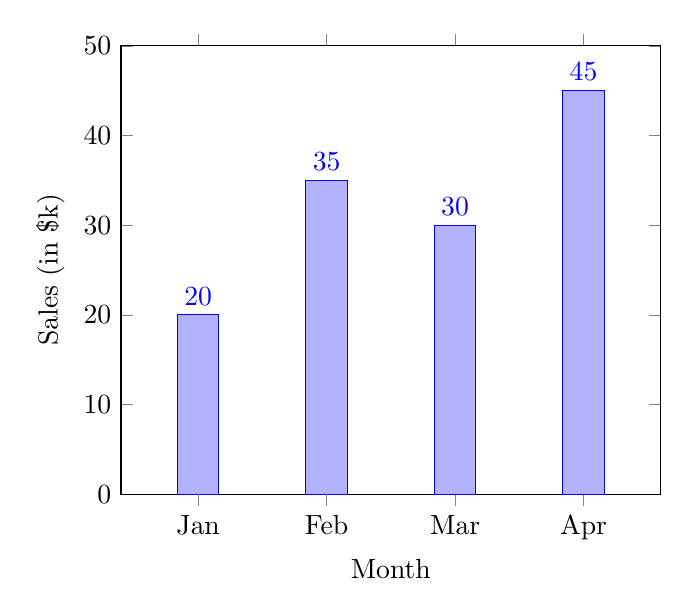
\begin{tikzpicture}
\begin{axis}[
    ybar,
    ylabel={Sales (in \$k)},
    xlabel={Month},
    symbolic x coords={Jan, Feb, Mar, Apr},
    xtick=data,
    nodes near coords,
    bar width=15pt,
    enlarge x limits=0.2,
    ymin=0, ymax=50
]
\addplot coordinates {(Jan, 20) (Feb, 35) (Mar, 30) (Apr, 45)};
\end{axis}
\end{tikzpicture}
\end{frame}

\begin{frame}{Trend Over Time (Line Chart)}
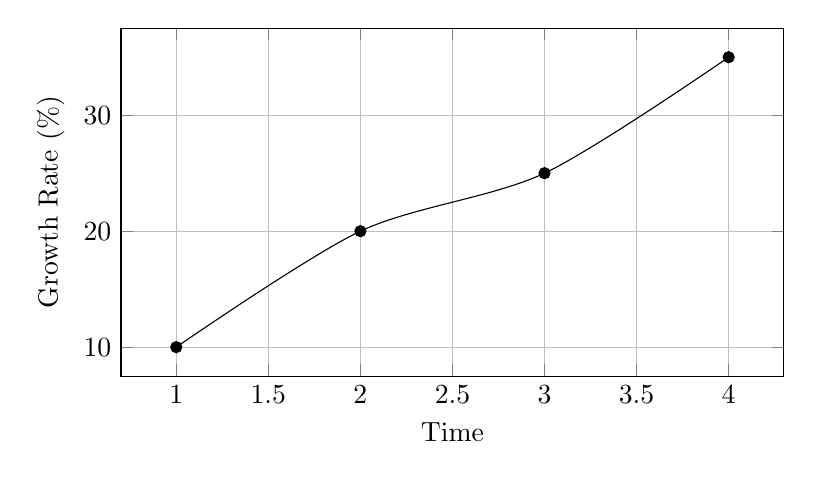
\begin{tikzpicture}
\begin{axis}[
    xlabel=Time,
    ylabel=Growth Rate (\%),
    grid=major,
    width=10cm,
    height=6cm
]
\addplot[smooth,mark=*] coordinates {(1,10) (2,20) (3,25) (4,35)};
\end{axis}
\end{tikzpicture}
\end{frame}

\begin{frame}{Market Share (Pie Chart)}
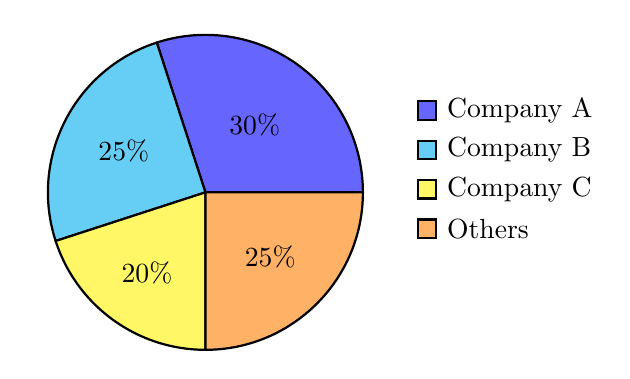
\begin{tikzpicture}
\pie[text=legend, radius=2]{
  30/Company A,
  25/Company B,
  20/Company C,
  25/Others
}
\end{tikzpicture}
\end{frame}

\begin{frame}{Animated Bar Chart: Quarterly Growth}
\begin{tikzpicture}
\begin{axis}[
    ybar,
    ymin=0,
    ymax=60,
    bar width=15pt,
    symbolic x coords={Q1, Q2, Q3, Q4},
    xtick=data,
    nodes near coords,
    enlarge x limits=0.2,
    ylabel={Revenue (in \$k)},
    xlabel={Quarter}
]

% Reveal one bar at a time using overlays <1>, <2>, etc.
\only<1>{
\addplot coordinates {(Q1, 20)};
}
\only<2>{
\addplot coordinates {(Q1, 20) (Q2, 35)};
}
\only<3>{
\addplot coordinates {(Q1, 20) (Q2, 35) (Q3, 40)};
}
\only<4>{
\addplot coordinates {(Q1, 20) (Q2, 35) (Q3, 40) (Q4, 50)};
}

\end{axis}
\end{tikzpicture}
\end{frame}

\begin{frame}{Animated Bar Chart: Quarterly Growth}
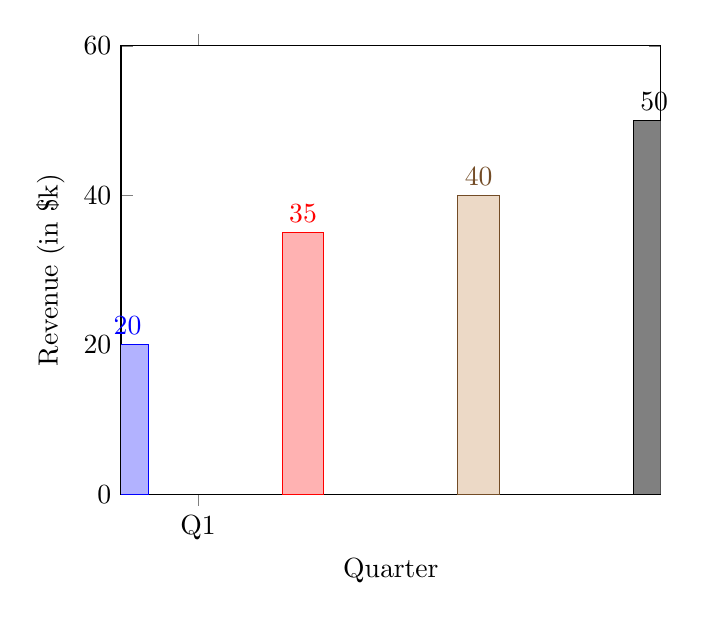
\begin{tikzpicture}
\begin{axis}[
    ybar,
    ymin=0,
    ymax=60,
    bar width=15pt,
    symbolic x coords={Q1, Q2, Q3, Q4},
    xtick=data,
    nodes near coords,
    enlarge x limits=0.2,
    ylabel={Revenue (in \$k)},
    xlabel={Quarter}
]

% Reveal one bar at a time using overlays <1>, <2>, etc.
\uncover<1>{
\addplot coordinates {(Q1, 20)};
}
\uncover<2>{
\addplot coordinates {(Q2, 35)};
}
\uncover<3>{
\addplot coordinates {(Q3, 40)};
}
\uncover<4>{
\addplot coordinates {(Q4, 50)};
}

\end{axis}
\end{tikzpicture}
\end{frame}


\begin{frame}{Using \textbackslash pause}
\begin{itemize}
    \item First item appears immediately
    \pause
    \item Second item appears after first click
    \pause
    \item Third item appears after second click
\end{itemize}
\end{frame}

% Slide using \uncover
\begin{frame}{Using \textbackslash uncover<n->}
\begin{itemize}
    \uncover<1->{\item This is always visible from step 1 onward}
    \uncover<2->{\item This appears on step 2 and stays visible}
    \uncover<3->{\item This appears on step 3}
\end{itemize}
\end{frame}

% Slide using \onslide
\begin{frame}{Using \textbackslash onsli{}de<n->}
\begin{itemize}
    \onslide<1->{\item Step 1: Introduction}
    \onslide<2->{\item Step 2: Explanation}
    \onslide<3->{\item Step 3: Conclusion}
\end{itemize}
\end{frame}

\end{document}